\section{Ejercicio 6}


Los Latches y los flip-flops son elementos utilizados en el alamcenaje de información. Cada uno puede guardar un bit de información. La diferencia principal entre ellos es que el latch chequea continuamente la entrada, cambiando la salida en caso de alguna variaci\'on en la entrada. Por otro lado, el flip-flop puede pensarse como la integración de un latch y un cicruito que responde a un clock, cambiando la salida no solo cuando la entrada varía, sino cuando incide un flanco del clock. En otras palabras, los latches son circuitos asincrónicos mientras que los flip-flops son circuitos sincrónicos. En general un flip-flop está compuesto por muchas más compuertas lógicas que un latch, por ende se esperaría que los tiempos de respuesta sean distintos. 




\subsection{Latch SR}

Un tipo común de latches es el latch $SR$, por set-reset. Su circuito es el siguiente:

\begin{figure}[H]
	\centering
	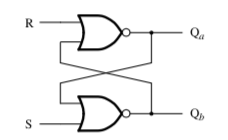
\includegraphics[width=0.5\textwidth]{Ejercicio6/Recursos/latchSR}
	\caption{Latch SR}
\end{figure}

Su tabla de verdad es como sigue:


\subsection{Flip-flop D}
Un tipo de flip-flop es el flip-flop tipo D, cuya salida copia la entrada $D$ cuando llegue un flanco de clock (puede configurarse el circuito para que sea ascendente o descendente). 

\begin{figure}[H]
	\centering
	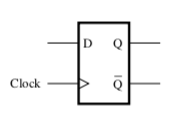
\includegraphics[width=0.5\textwidth]{Ejercicio6/Recursos/flipflopD}
	\caption{Flip-flop D}
\end{figure}

Un dispositivo de este estilo puede dividirse en dos partes, una que responde a cambios en el clock, y otra que almacena la información, en otras palabras un latch. El circuito siguiente es una configuración posible para la realización de un flip-flop tipo D:

\begin{figure}[H]
	\centering
	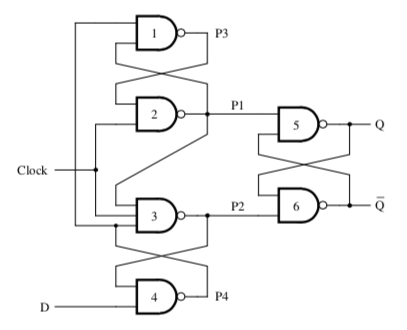
\includegraphics[width=0.6\textwidth]{Ejercicio6/Recursos/flipflopDcircuito}
	\caption{Circuito flip-flop D}
\end{figure}

\subsection{Mediciones}

En la siguiente tabla se resumen los resultaods obtenidos, as\'i como los vaores comerciales de coparaci\'on:

\begin{table}[H]
\begin{tabular}{llll}\hline
\multicolumn{1}{c}{}           & \multicolumn{1}{c}{Hold time (ns)} & \multicolumn{1}{c}{Set-up time (ns)} & Propagation Delay (ns) \\
\hline
Latch SR comercial (HC 373)    & 10                                 & 10                                   & 15-30                  \\
Latch SR implemenado           & 19                              &   17                                   &  44                \\
Flip-Flop D comercial (CD4013) & 2-5                                & 10-20                                & 65-130                 \\
Flip-Flop D implementado       &    

                                &                                      &                        \\  \hline
\end{tabular}
\end{table}
